\chapter{DOKUMENTASI PENGAMBILAN DATA}
\begin{figure}[!htbp]
    \centering
    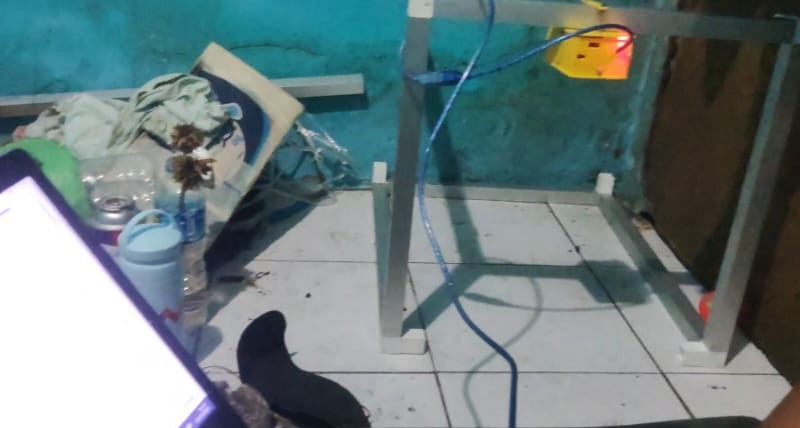
\includegraphics[width=0.5\linewidth]{images/Proses-Akuisisi-Data.jpeg}
    \caption{pengambilan data}
    \citep{ajitot2024koefisien}
    \label{fig:pengambilan-data}
\end{figure}
\begin{figure}[!htbp]
    \centering
    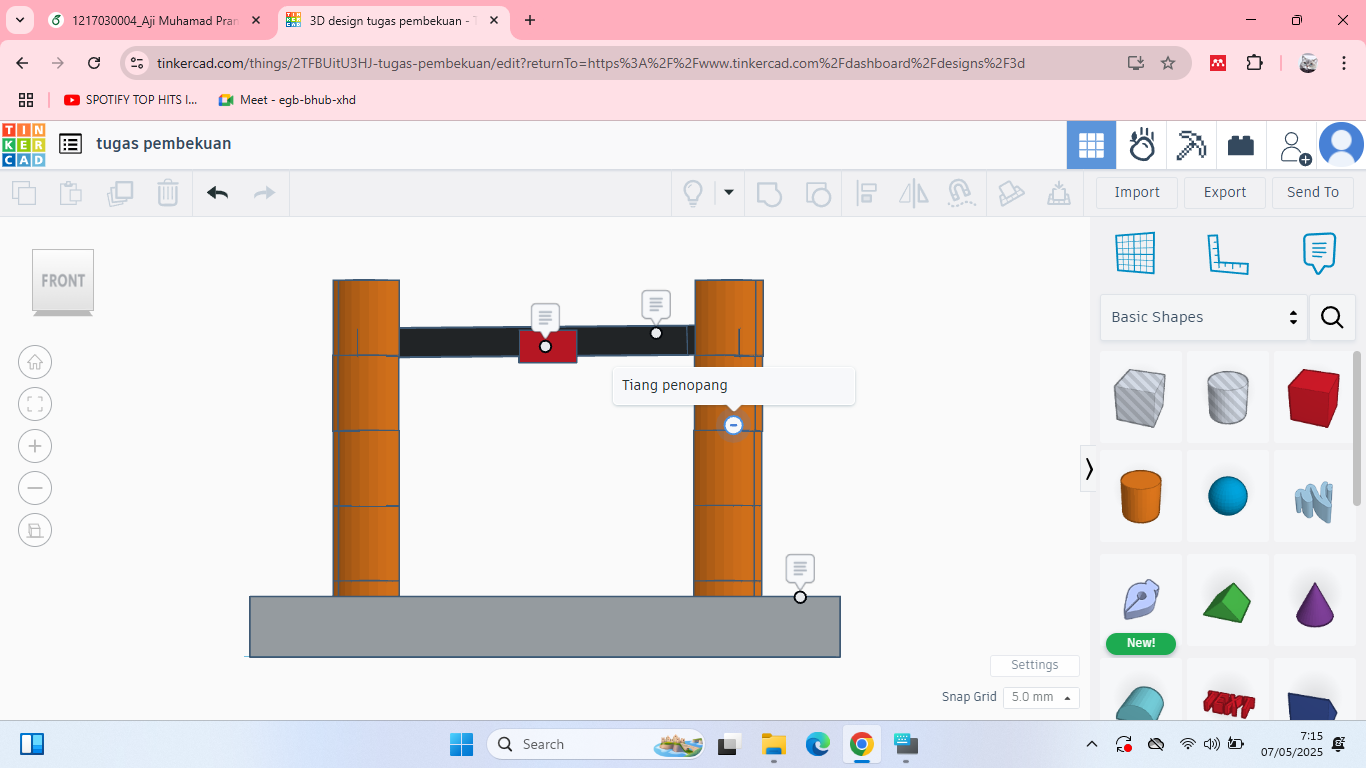
\includegraphics[width=0.5\linewidth]{images/Screenshot (2).png}
    \caption{Ilustrasi alat}
    \label{fig:ilustrasi-alat-1}
\end{figure}
\begin{figure}[!htbp]
    \centering
    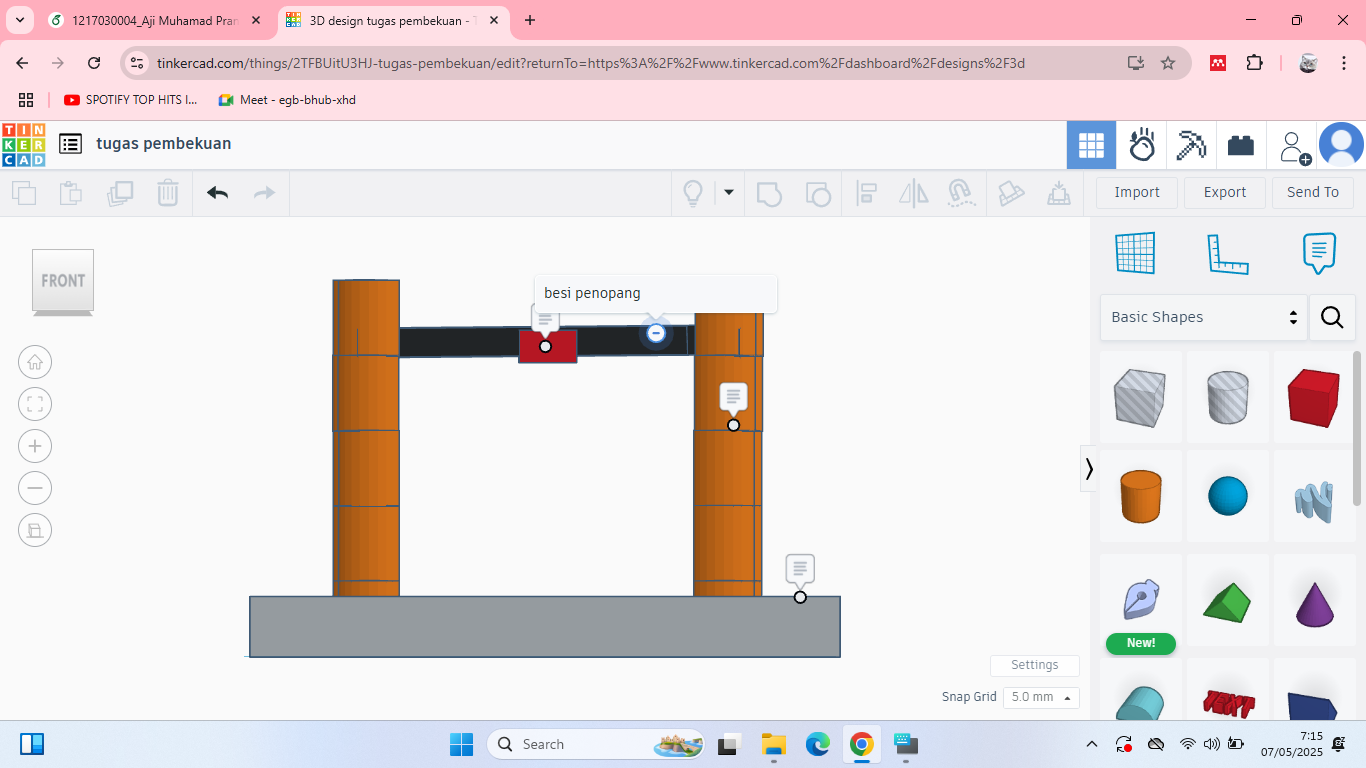
\includegraphics[width=0.5\linewidth]{images/Screenshot (3).png}
    \caption{Ilustrasi alat}
    \label{fig:ilustrasi-alat-2}
\end{figure}
\begin{figure}[!htbp]
    \centering
    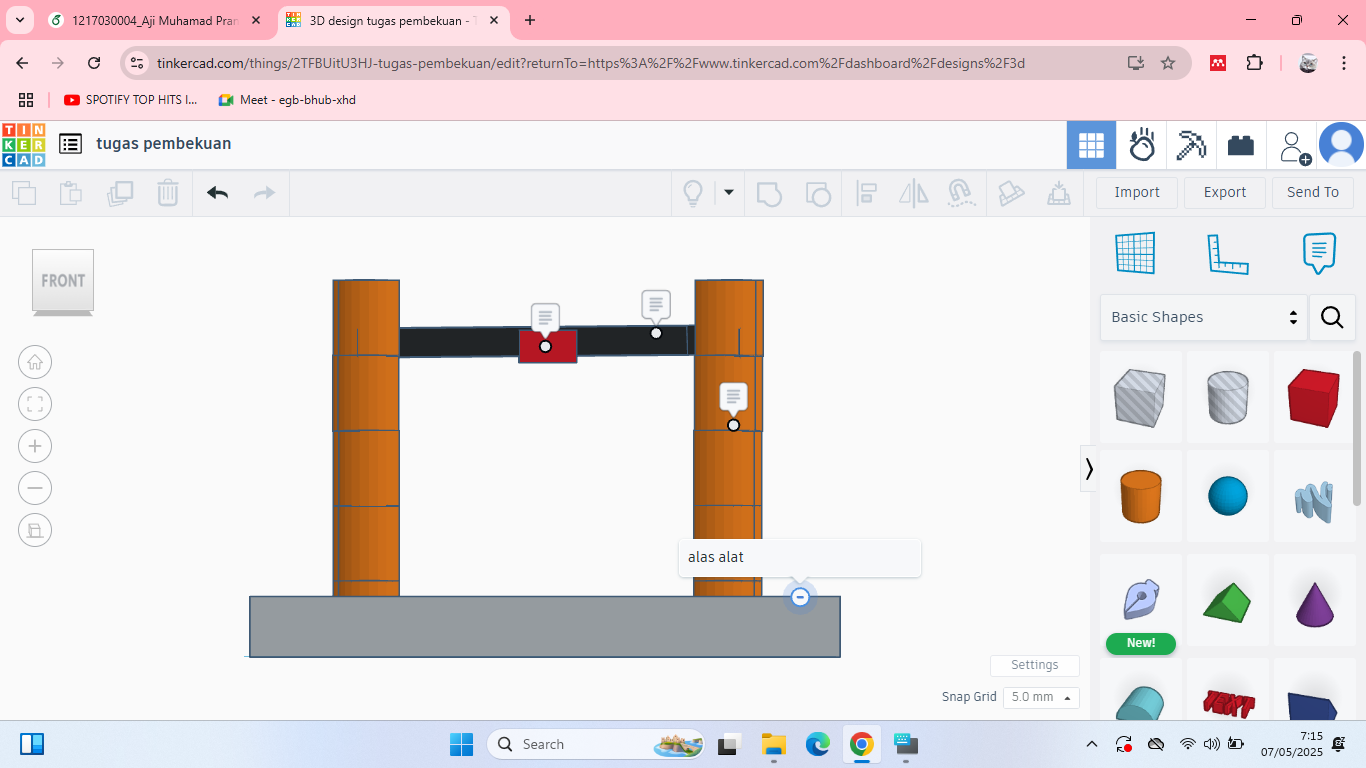
\includegraphics[width=0.5\linewidth]{images/Screenshot (4).png}
    \caption{Ilustrasi alat (tampak depan)}
    \label{fig:ilustrasi-alat-depan}
\end{figure}
\begin{figure}[!htbp]
    \centering
    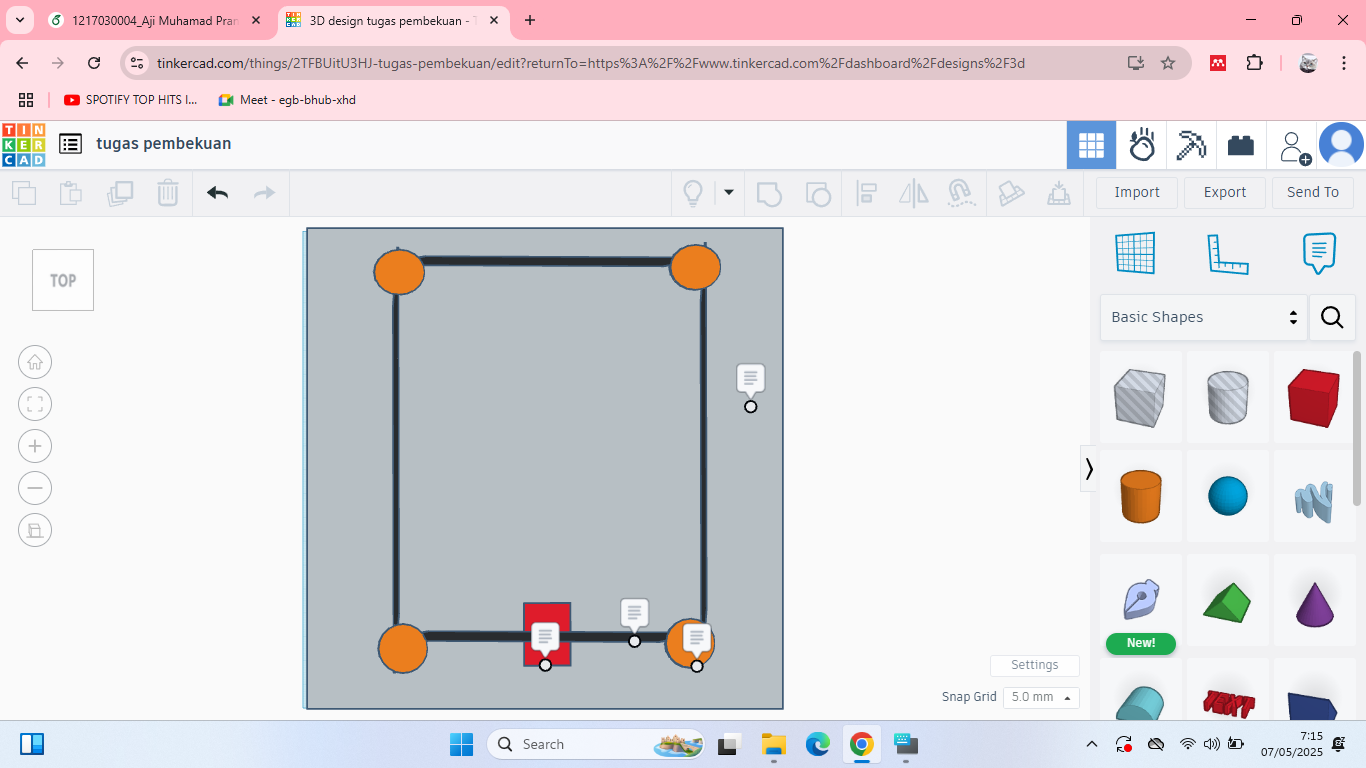
\includegraphics[width=0.5\linewidth]{images/Screenshot (5).png}
    \caption{Ilustrasi alat(tampak atas)}
    \label{fig:ilustrasi-alat-atas}
\end{figure}

